\subsection{Case Study}
\label{sec:eval}

We now demonstrate the application of our optimization framework in a
case study.  Specifically, we use it to study the placement of a 100MW
datacenter and wind farm in the New England transmission network.
Instead of specifying a desired capacity for the wind farm, we assume
that we want sufficient wind energy to completely offset the energy
consumption of the datacenter (making the size of the wind farm
dependent on the locations of both the datacenter and the wind farm).
% This scenario corresponds to when a company wants to build a new
% datacenter, and a corresponding wind farm to offset the energy use of
% the datacenter.

\subsubsection{Instantiating the framework parameters}

The production of wind power and datacenter cooling both depend on weather conditions.  Thus, we obtained Typical Meteorological Year (TMY) information for 56 locations in the U.S. New England area as shown in Figure~\ref{fig:NE_locs}.  A TMY is a 1-year dataset of hourly weather values selected to include a representative range of weather phenomena for a location, while still giving annual averages that are consistent with the long-term averages for the location.  The TMY data is obtained from US Department of Energy.\footnote{\url{http://apps1.eere.energy.gov/buildings/energyplus/weatherdata about.cfm}} We use the TMY wind speeds and air pressures, conversion losses, and specifications for the 1.5MW Series wind turbine from General Electric Company \cite{GE15MW} to compute $\beta(l,t)$ at each location $l$ during time epoch $t$.

\begin{figure}[ht]
\centering
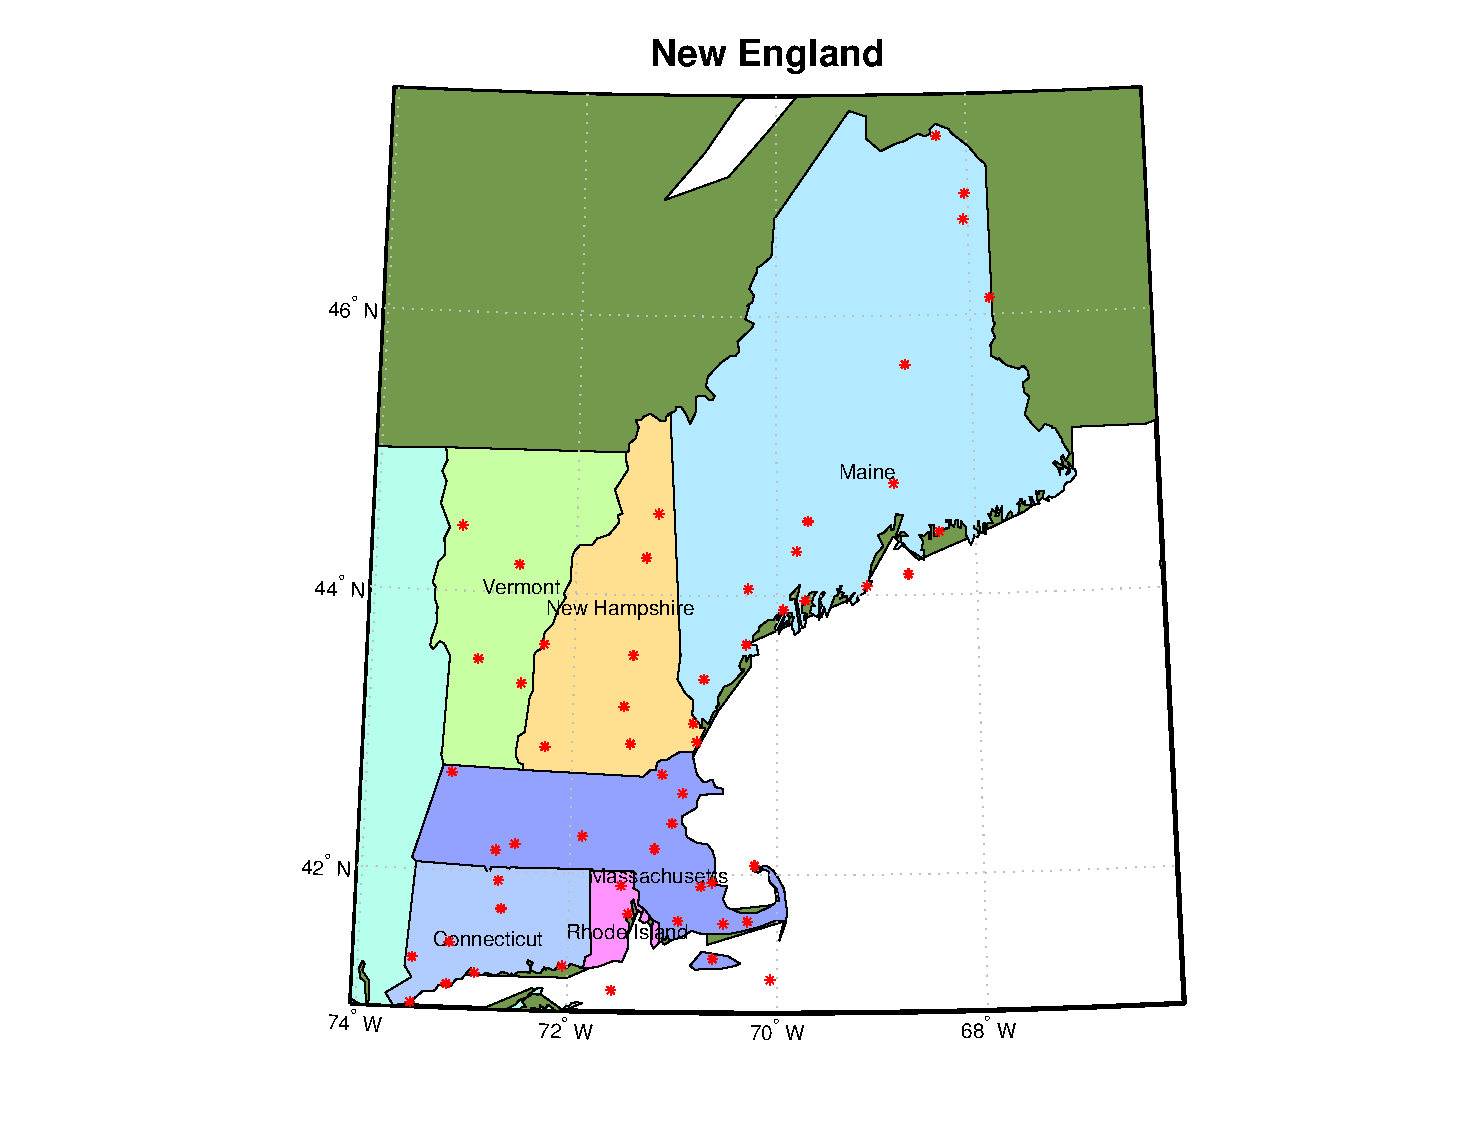
\includegraphics[width=1\columnwidth]{img/NE_map}
\caption{Candidate locations in New England}
\label{fig:NE_locs}
\end{figure}

We adopt the values and approaches for computing PUE, datacenter
construction costs, wind farm construction costs, land costs,
transmission lines and network connection costs, and grid energy costs
from \cite{berral2014building}.  Table \ref{tab:loc-dependent-pars}
shows part of the location-dependent parameters for five typical
locations used in our experiments, and Table \ref{tab:constant-pars}
shows the values of the location-independent parameters.  Datacenter
construction costs are financed and amortized across 12 years.  Wind
farm construction costs are financed over 12 years and amortized over
24 years.  We assume that land cost is fully recoverable, so that the
only incurred cost is that of financing, spread over 12 years.
Finally, the cost for IT equipment is financed and amortized over 4
years.  For financing, we use an annual interest rate of 3.25\%.

\begin{table}[ht]
\begin{center}
\caption{Location-dependent parameter settings for five typical
  locations.  \thunote{Xiaoying, the maxPUE cannot possibly be that
    low, can it?}}
\begin{tabular}{|l|p{22pt}|p{28pt}|p{20pt}|p{27pt}|p{27pt}|}
\hline
\textbf{Locations}& Burlinton, NH&Springfield Hartnes, VT&Nash Island, CO&Marthas Vineyard, RI & Mount Washington, NH
\\
\hline
$pLand$ (\$/m$^2$)&946.9&946.9&946.9&680.21&946.9  \\
$maxPUE$&1.0650&1.0639&1.0698&1.0639&1.0601 \\
$cLinePow$ (M\$)&64.5&77.2&16.6	&86.6&107.1 \\
$cLineNet$ (M\$)&13.5&16.7&16.9&17.7&21.3 \\
$pEnergy$ (\$/kWh)&0.0941&0.0941&0.1281&	0.1281&	0.1257 \\
Average $\beta$ (\%) &11.7&2.7&	40&	15.9&56.8 \\
\hline
\end{tabular}
\label{tab:loc-dependent-pars}
\end{center}
\end{table}

\begin{table}[ht]
\begin{center}
\caption{Values of location-independent parameters.}
\begin{tabular}{|l|c|r|}
\hline
\textbf{Parameter}& \textbf{Value} &\textbf{Unit}\\
\hline
$dcArea$ &	0.557& m$^2$/kW \\
$\textit{pBuildDC}$&12000& \$/kW	 \\
$serverPow$ 	&0.275&kW/serv \\
$switchPow$ 	&0.48 &kW/switch\\
$servsSwitch$ &	32 &servs/switch\\
$pServer$ 	&2000 &\$/serv\\
$pSwitch$  & 20000 &\$/switch\\
$\textit{pNBWServ}$&	1 & \$/serv-month\\
$wfArea$ &	18.21 &\$/m$^2$\\
$\textit{pBuildWF}$&	2.1& \$/kW \\

\hline
\end{tabular}
\label{tab:constant-pars}
\end{center}
\end{table}



\thunote{Xiaoying, you may have replied via email, but could you put
  in the assumed grid load?} For each time epoch $t$, we compute the
wind energy being generated by all the wind farms (existing ones and
the new one being placed) using $\beta(l,t)$.  We assume full loading
of all datacenters (existing ones and the new one being placed.  We
then compute the system loss for the time epoch for the placement of
the new datacenter and wind farm at locations $d$ and $w$,
respectively, using the simulation approach described in
Section~\ref{sec:quantify}.  We map the candidate locations in
Figure~\ref{fig:NE_locs} to buses using the approach previously
discussed in Section~\ref{sec:quantify}.  For each possible pair of
($d$, $w$), we sum the transmission loss over the entire year.

Finally, we set $pTransLoss$ to the maximum electricity price in the
whole area.

\subsubsection{Placement approaches}

To see the impact of considering transmission loss, as well as the simultaneous placement of datacenter and wind farm, we compare results for five different placement approaches:

\textbf{DC\_WF\_OPT:} This strategy individually looks for the best location to put the datacenter and the wind farm; i.e., it solves the optimization problem for the datacenter without considering the new wind farm, and then solves the optimization problem again for the wind farm without considering the new datacenter.  This strategy also ignore transmission loss.

\textbf{DC+G\_WF+G:} This strategy is the same as DC\_WF\_OPT except that transmission loss is considered when solving the optimization problem.

\textbf{Min\_Loss:} This strategy finds locations for the datacenter and wind farm that minimizes the cost of transmission loss.

\textbf{Co-location:} This strategy assumes that the datacenter and wind farm
should be co-located, and so finds a single location for both that minimizes the overall cost.

\textbf{Jointly:} This strategy considers the simultaneous placement of the datacenter and wind farm, and uses all of the costs and revenues in the optimization framework.

\subsubsection{Results}
Figure \ref{fig:cost1dc1wf} shows the resulting total cost when using
the five different placement strategies.  It is easy to see that not
considering transmission system losses (DC\_WF\_OPT), considering only
transmission system losses (Min\_Loss), and forcing the co-location of
the datacenter and wind farm all lead to higher total costs.
Specifically, DC\_WF\_OPT incurs the highest transmission cost,
Min\_Loss incurs high cost for laying networking lines, and
Co-location incurs high energy cost.  In comparison, considering both
transmission system loss and datacenter construction/operation costs
can lead to finding locations that best balance these factors, leading
to lowest overall cost.

\thunote{We cannot use this \$663M as the baseline.  Use the
  co-location as the baseline.}
We calculate all of the combinations for wind farm and datacenter
locations and use the average total cost of these combinations (which
is \$663M per year) as the baseline for comparison. Then, the
locations found and the corresponding cost savings of the five
strategies are listed in Table \ref{tab:costsaving}.

\begin{figure}[ht]
\centering
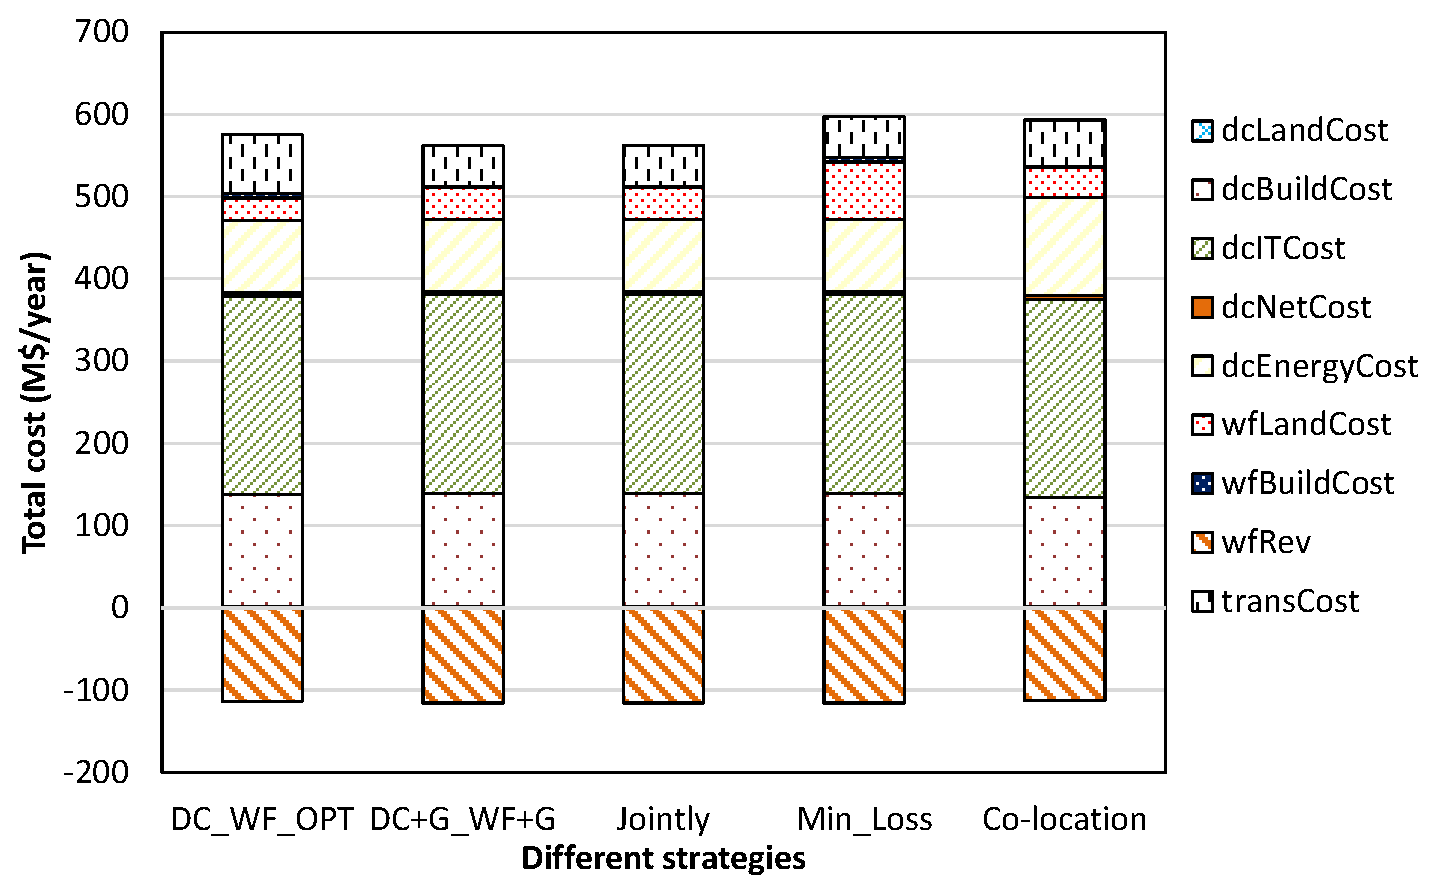
\includegraphics[width=1\columnwidth]{img/cost-one-dc-one-wf}
\caption{Costs of building one datacenter (100MW) with one wind farm}
\label{fig:cost1dc1wf}
\end{figure}

\begin{table}[ht]
\begin{center}
\caption{Detailed results of cost savings by different strategies.}
\begin{tabular}{|l|p{50pt}|p{50pt}|p{30pt}|p{20pt}|}
\hline
\textbf{Strategy}& \textbf{Datacenter location} &\textbf{Wind farm location} &\textbf{Total cost (M\$/year)} &\textbf{Cost saving (\%)} \\
\hline
\textbf{DC\_WF\_OPT} &  Burlington,NH  & Mount Washington, NH & 461.5& 30.4 \\
\textbf{DC+G\_WF+G} &Springfield Hartnes, VT  & Nash Island, CO& 446.2& 32.7\\
\textbf{Jointly} &Springfield Hartnes, VT&  Nash Island, CO & 446.2 & 32.7\\
\textbf{Min\_Loss} &Springfield Hartnes, VT & Marthas Vineyard, RI & 481.5 & 27.4 \\
\textbf{Co-location}& Nash Island, CO &Nash Island, CO& 480.7 & 27.5  \\
\hline
\end{tabular}
\label{tab:costsaving}
\end{center}
\end{table}

%%% Local Variables:
%%% mode: latex
%%% TeX-master: "paper"
%%% End:
